\subsection{Read Access Time and Energy}

\begin{figure}[!t]
\centerline
{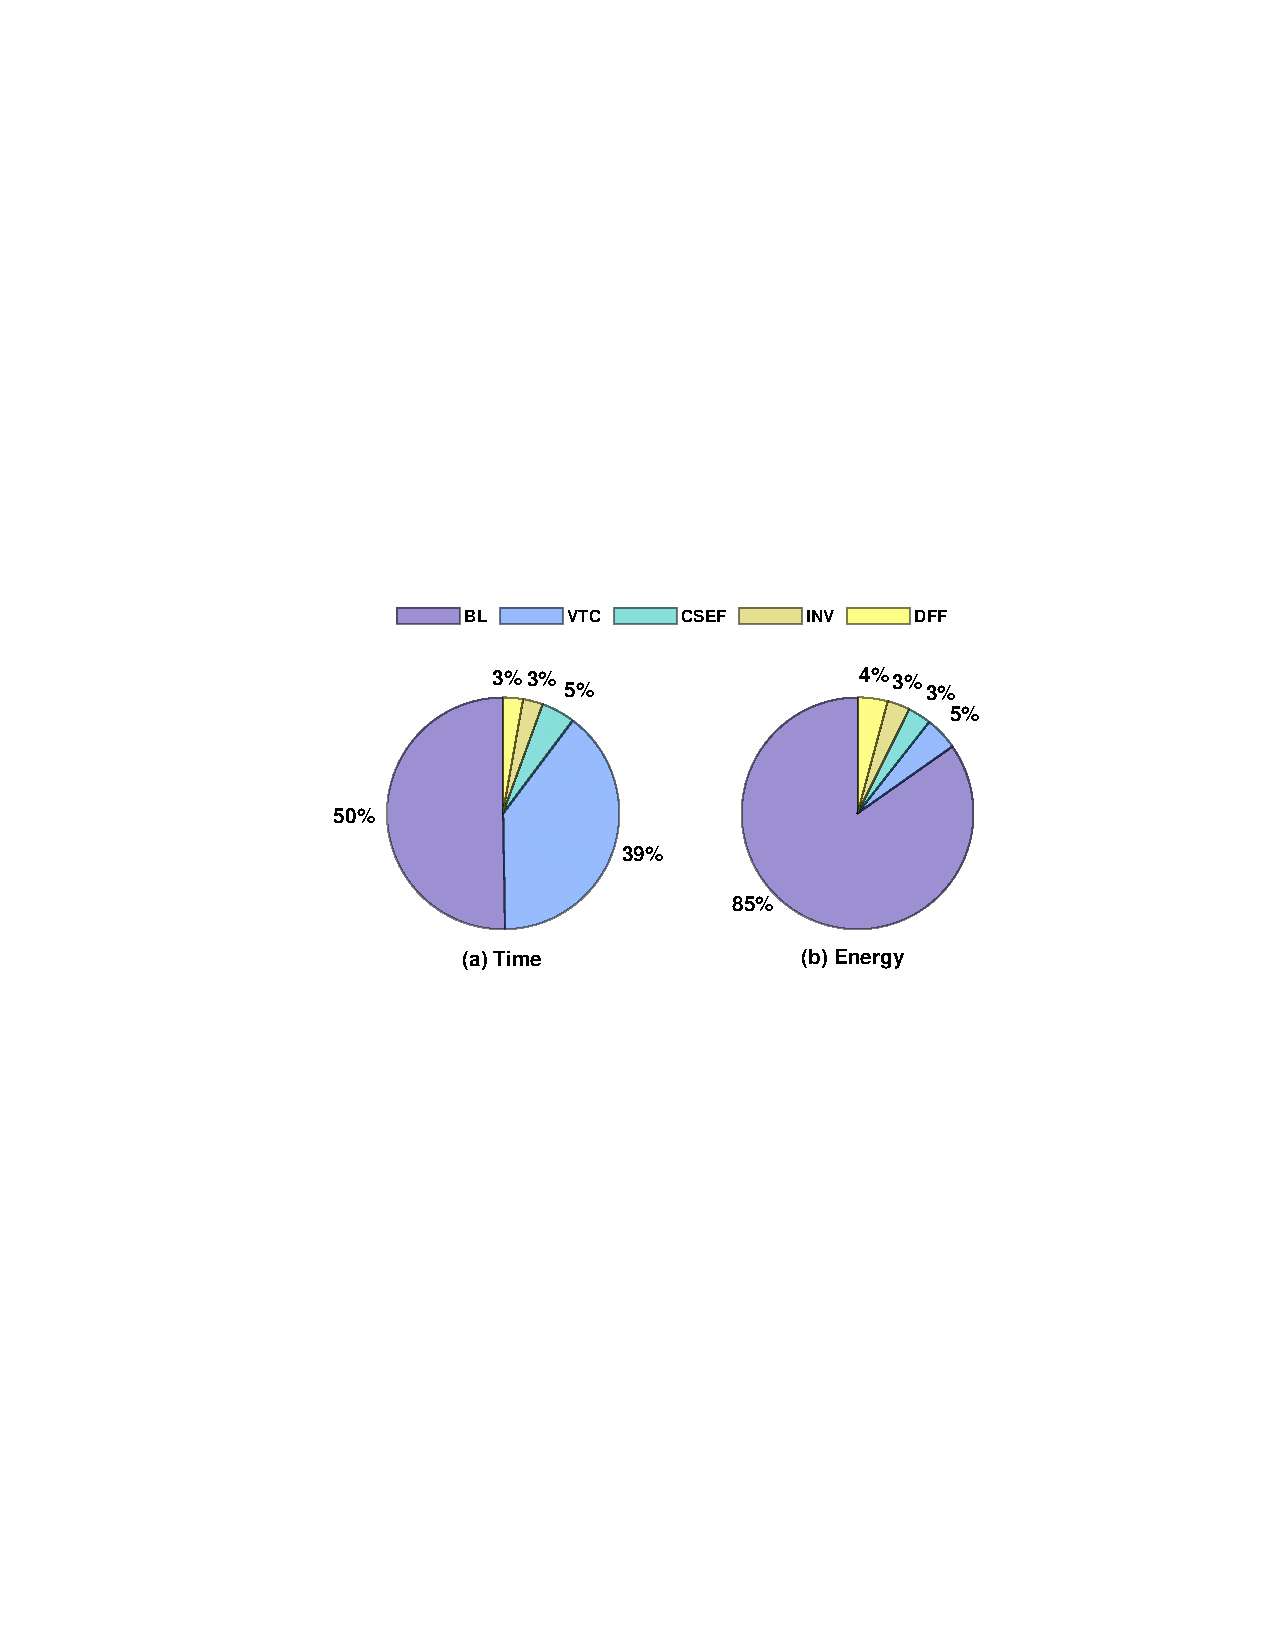
\includegraphics[width=0.46\textwidth]{fig/time_energy_pie_new.pdf}}
\caption{Breakdown of (a) read access time and (b) energy under supply voltage of 1.2 V.}
\label{fig_time_energy_pie}
\end{figure}

To evaluate the overall performance of the proposed TSA, we designed a typical sub-bank size of $512\times512$ 1T1R bitcells with 16:1 column multiplexing for the readout circuit, where each TSA is shared by 16 columns. The simulations are performed under the adopted 40-nm technology, as mentioned in Section \ref{sim_model}. 

In each read cycle, the overall read access time $T_{read}$ is divided into the time of $T_{reset}$ to precharge the bitline voltage $V_{BL}$ and the time of $T_{DISCH}$ associated with the VTC and state detection. 
%$T_{read}$ is set by the time $T_{PRE}$ to charge the bitline voltage $V_{BL}$ to precharge voltage $V_{PRE}$, and the sensing delay $T_{sense}$ associated with the sense amplifier.  
$T_{DISCH}$ is equal to the summation of the time of the delay line $T_1$ ($T_1 + T_2 + T_3$) for single-level (multi-level) sensing schemes and the PGI enable time $\Delta T$, as shown in Fig. \ref{fig_prop_circuit} (Fig. \ref{fig_multiple_sensing}). 
In this work, $T_{reset}$ and $T_{DISCH}$ are equal since they represent the positive half and negative half of the clock signal generated by the timing control loop. 
% The clock period is designed as 10 ns to set the read frequency to 100 MHz. So the sensing time ($T_{DISCH}$) is 5 ns, which is enough to develop bitline voltage and discriminate $V_C$ accurately according to Fig. \ref{fig_ber_delay}. 
The size of the precharge NMOS transistor is determined by the bitline parasitic capacitors $C_{BL}$ and precharge voltage $V_{PRE}$ under the given precharge time.
% It is to be noted that the precharge time $T_{PRE}$ depends on the bitline parasitic capacitors $C_{BL}$ and the size of the precharge NMOS transistor.
The breakdown of the read access time is shown in Fig. \ref{fig_time_energy_pie}(a). The bitline precharge time takes 50\% of the read access time, and another 39\% is taken by the transition of $V_C$ after the VTC is enabled. Bitline precharge and VTC transition account for the major proportion of the total time. The CSEF occupies 5\% of the time to avoid the charge sharing-induced error and expand the read margin efficiently. The shaping inverters and the DFF latch take 3\% of the time equally. 

The read access energy consumed by the proposed TSA comprises four components that can be expressed as 
\begin{align}
\label{eq_energy}
E_{read} \approx E_{BL}+E_{VTC}+E_{CSEF}+E_{INV}+E_{DFF}
\end{align}
where $E_{BL}$ is the energy to precharge the bitline, $E_{VTC}$ is the energy consumed by the VTC, $E_{CSEF}$ is the energy drawn by the CSEF. $E_{INV}$ is the energy drawn by the PGI and the subsequent inverter to shape the signal. $E_{DFF}$ is the energy consumed by the DFF latch. The energy taken by the delay line is neglected in Eq. \eqref{eq_energy}, considering the fact that the delay line is shared by all the bitlines being read simultaneously.
As shown in Fig. \ref{fig_ber_delay}, the read access energy per bit is 49 fJ and 43 fJ under supply voltage of 1.2 V for HRS and LRS respectively. The total energy consumption breakdown is illustrated in Fig. \ref{fig_time_energy_pie}(b). Precharging the bitline consumes the vast majority, to be specific, 85\% of the total energy. The rest are almost equally contributed by the VTC, CSEF, INV and DFF, respectively. 
The energy-efficient shaping inverters benefit from the power gating technique.

% \begin{figure}[!t]
% \centerline
% {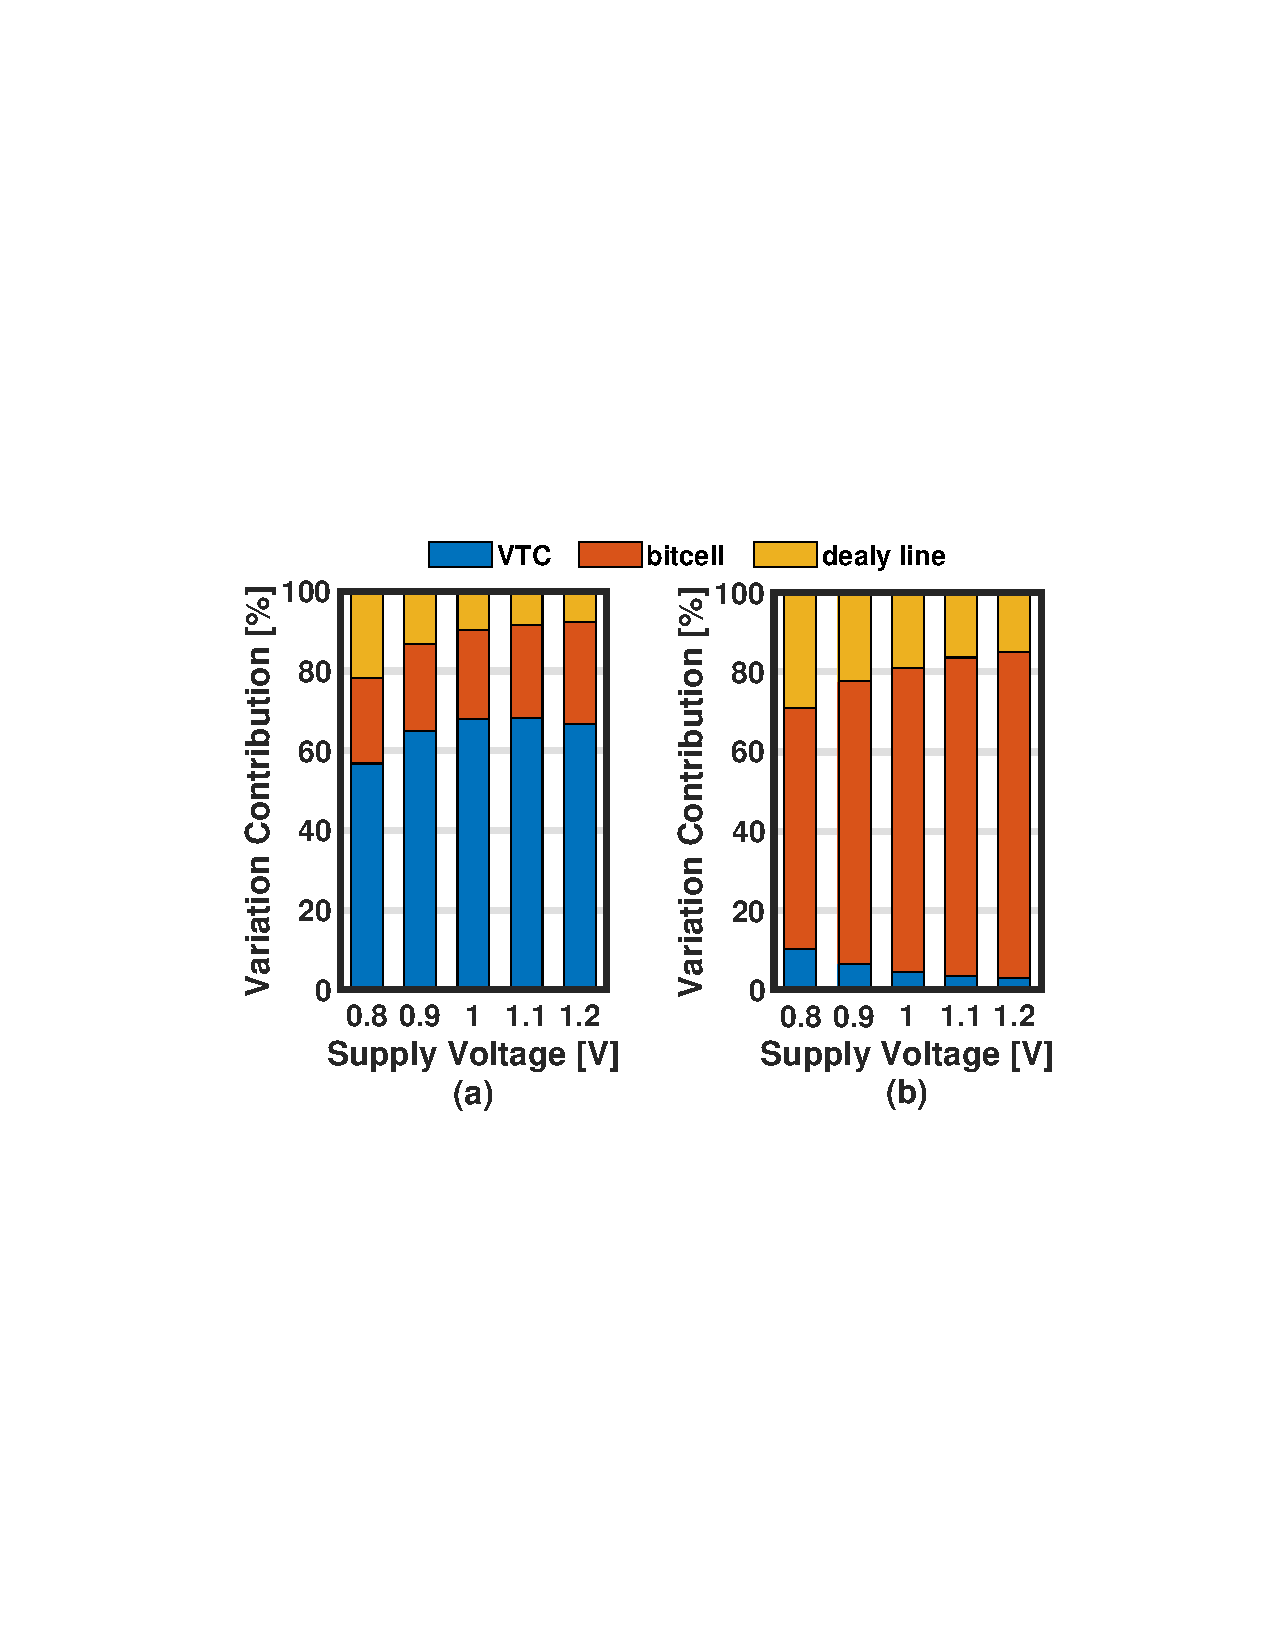
\includegraphics[width=0.45\textwidth]{fig/variation_with_vdd.pdf}}
% \caption{Variation contribution of the TSA when RRAM is in (a) HRS and (b) LRS with different supply voltage.}
% \label{fig_variation_with_vdd}
% \end{figure}

% \begin{figure}[!t]
% \centerline
% {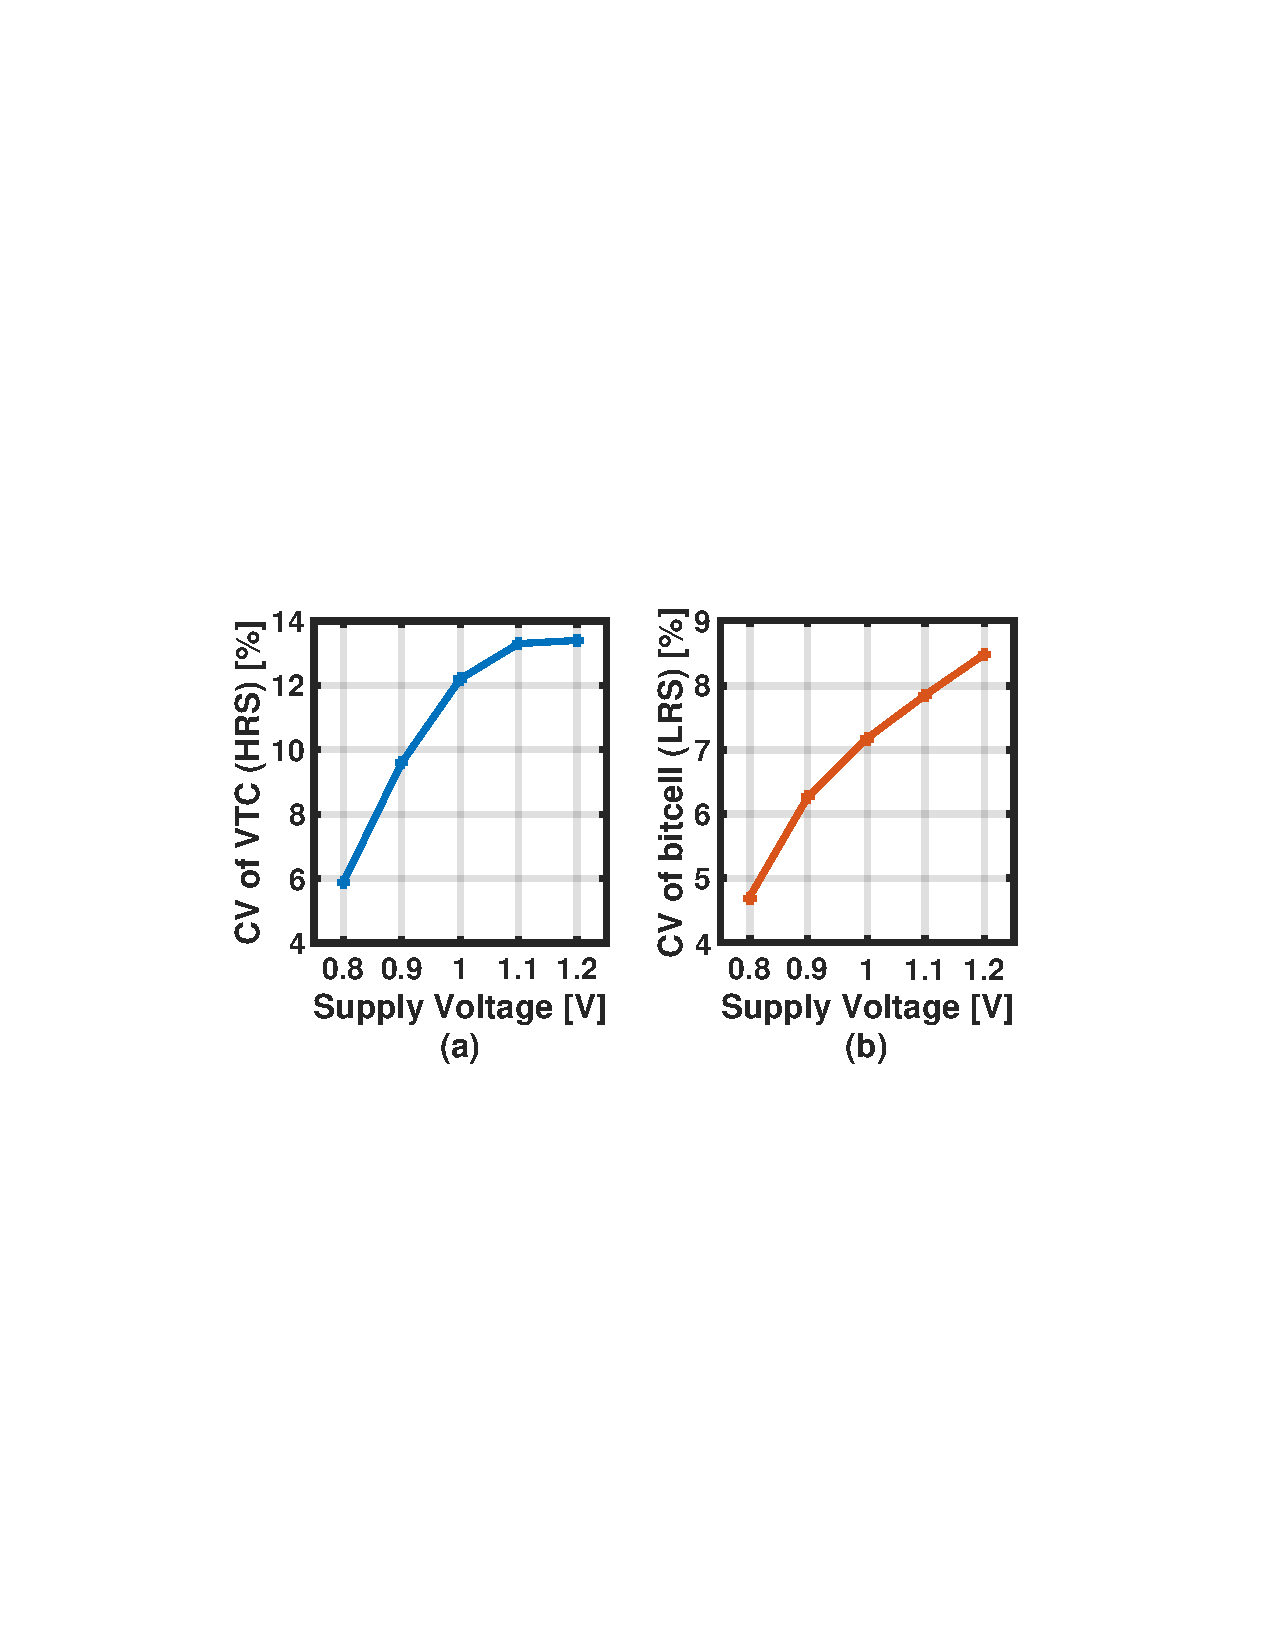
\includegraphics[width=0.45\textwidth]{fig/variation_with_vdd_absolute.pdf}}
% \caption{The coefficient of variation of (a) VTC when RRAM is in HRS and (b) bitcell when RRAM is in LRS with respect to supply voltage.}
% \label{fig_variation_with_vdd_abs}
% \end{figure}

\begin{figure}[!t]
     \centering
     \begin{subfigure}[(b)]{0.44\textwidth}
         \centering
         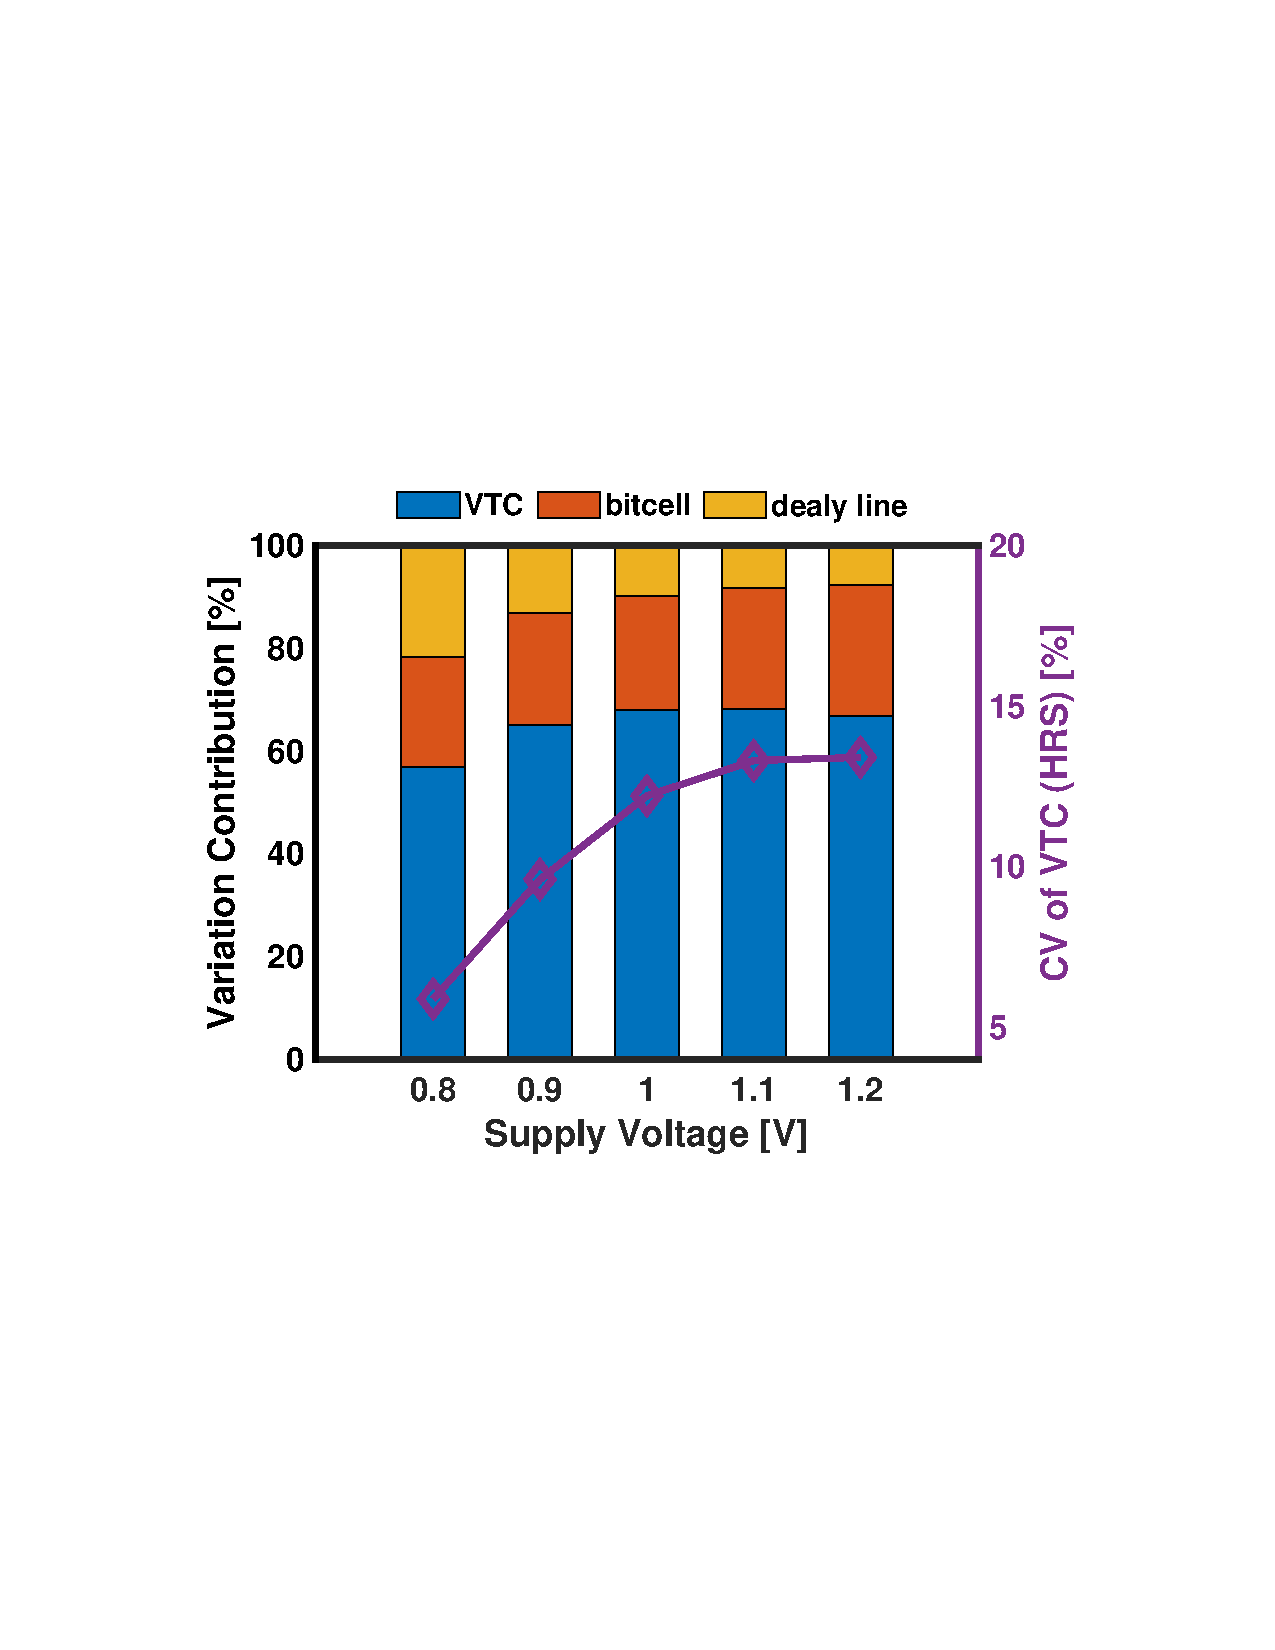
\includegraphics[width=0.9\textwidth]{fig/variation_hrs.pdf}
         \caption{}
         \label{fig_variation_hrs}
     \end{subfigure}
     \par\smallskip 
     \begin{subfigure}[b]{0.44\textwidth}
         \centering
         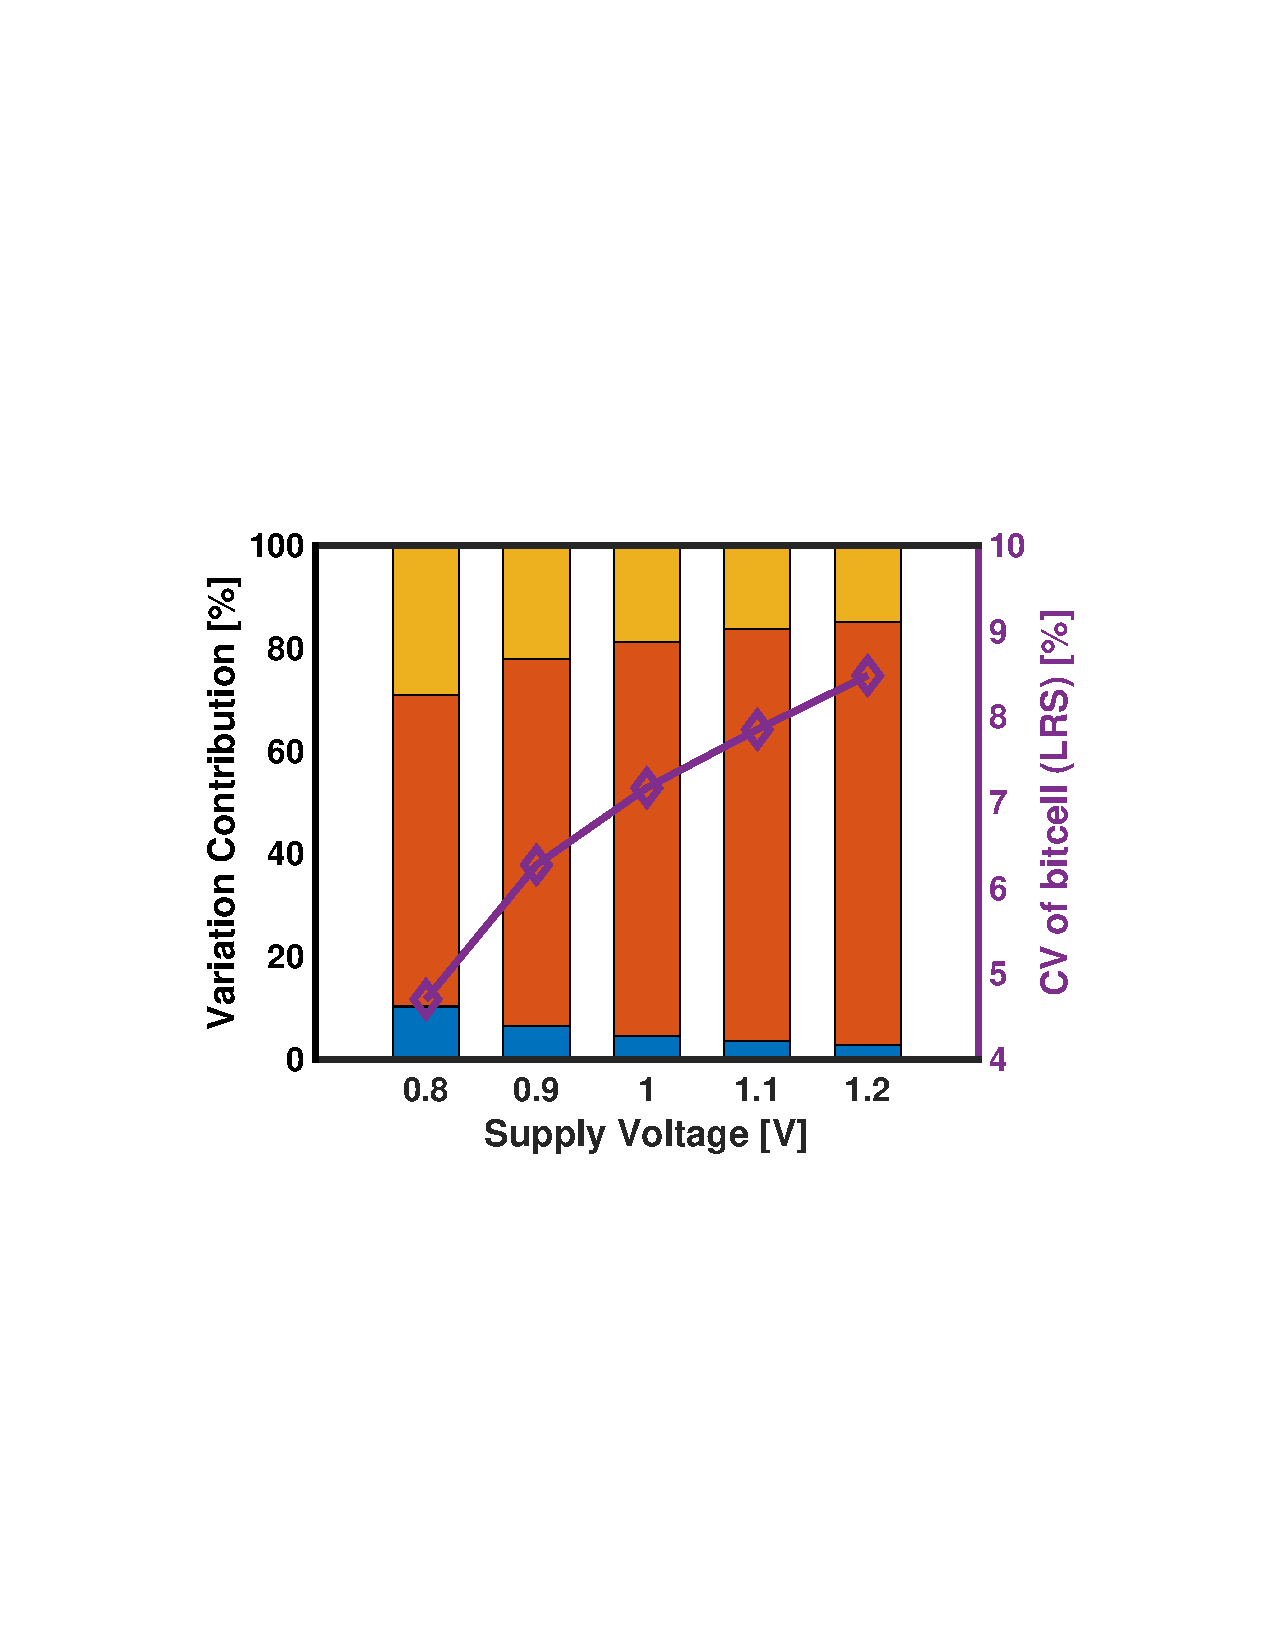
\includegraphics[width=0.9\textwidth]{fig/variation_lrs.pdf}
         \caption{}
         \label{fig_variation_lrs}
     \end{subfigure}
     
     \caption{Variation contribution of the TSA and the coefficient of variation (CV) of the major factor under different supply voltages when the RRAM is in (a) HRS and (b) LRS. The major contributors are VTC and bitcell respectively.}
     \label{fig_variation_with_vdd}
\end{figure}


\subsection{Robustness and Trade-offs}

To study the individual contributors to the overall variations, MC simulations are performed by enabling each block of the proposed TSA respectively. Fig. \ref{fig_variation_with_vdd} reports the variations contributed by the three main sources (i.e., VTC, the bitcell, and the delay line) versus the supply voltage. 
When the RRAM is in HRS, the VTC block is the dominant contributor to the variation, accounting for approximately $60 \sim 70\%$ under different supply voltage, as shown in Fig. \ref{fig_variation_hrs}. That is because the pull-down current, in this case, is relatively large and the output $V_C$ is charged from $V_{DD}$ to a lower voltage close to zero with variations. The bitline voltage almost keeps at the precharge voltage because of the high resistance of RRAM, resulting in a small variation ($\approx 20\%$). To evaluate the absolute variation of the major factor, the coefficient of variation (CV, which is defined as $\sigma/\mu \times 100$) of VTC when RRAM is in HRS is plotted in Fig. \ref{fig_variation_hrs} as well. The VTC variation increases with supply voltage and tends to be saturated when the supply voltage is higher than 1.1V.

When the RRAM is in LRS, the bitline will be discharged by the bitcell current, which is determined by both the low resistance of the RRAM device and the NMOS transistor, making the bitcell variation the dominant contribution ($\approx 60 \sim 80\%$), as shown in Fig. \ref{fig_variation_lrs}. In contrast, the variation of VTC is minimal ($\leq 10\%$) because $V_C$ almost keeps constant in this case. The CV of bitcell when the RRAM is in LRS is plotted in Fig. \ref{fig_variation_lrs} as well. The bitcell variation also increases with supply voltage, but overall, the variation contributed by bitcell when the RRAM is in LRS is lower than that by VTC when the RRAM is in HRS.
% The dominant contributions for the variation in HRS and LRS are the VTC and bitcell, respectively.


\begin{figure}[!t]
\centerline
{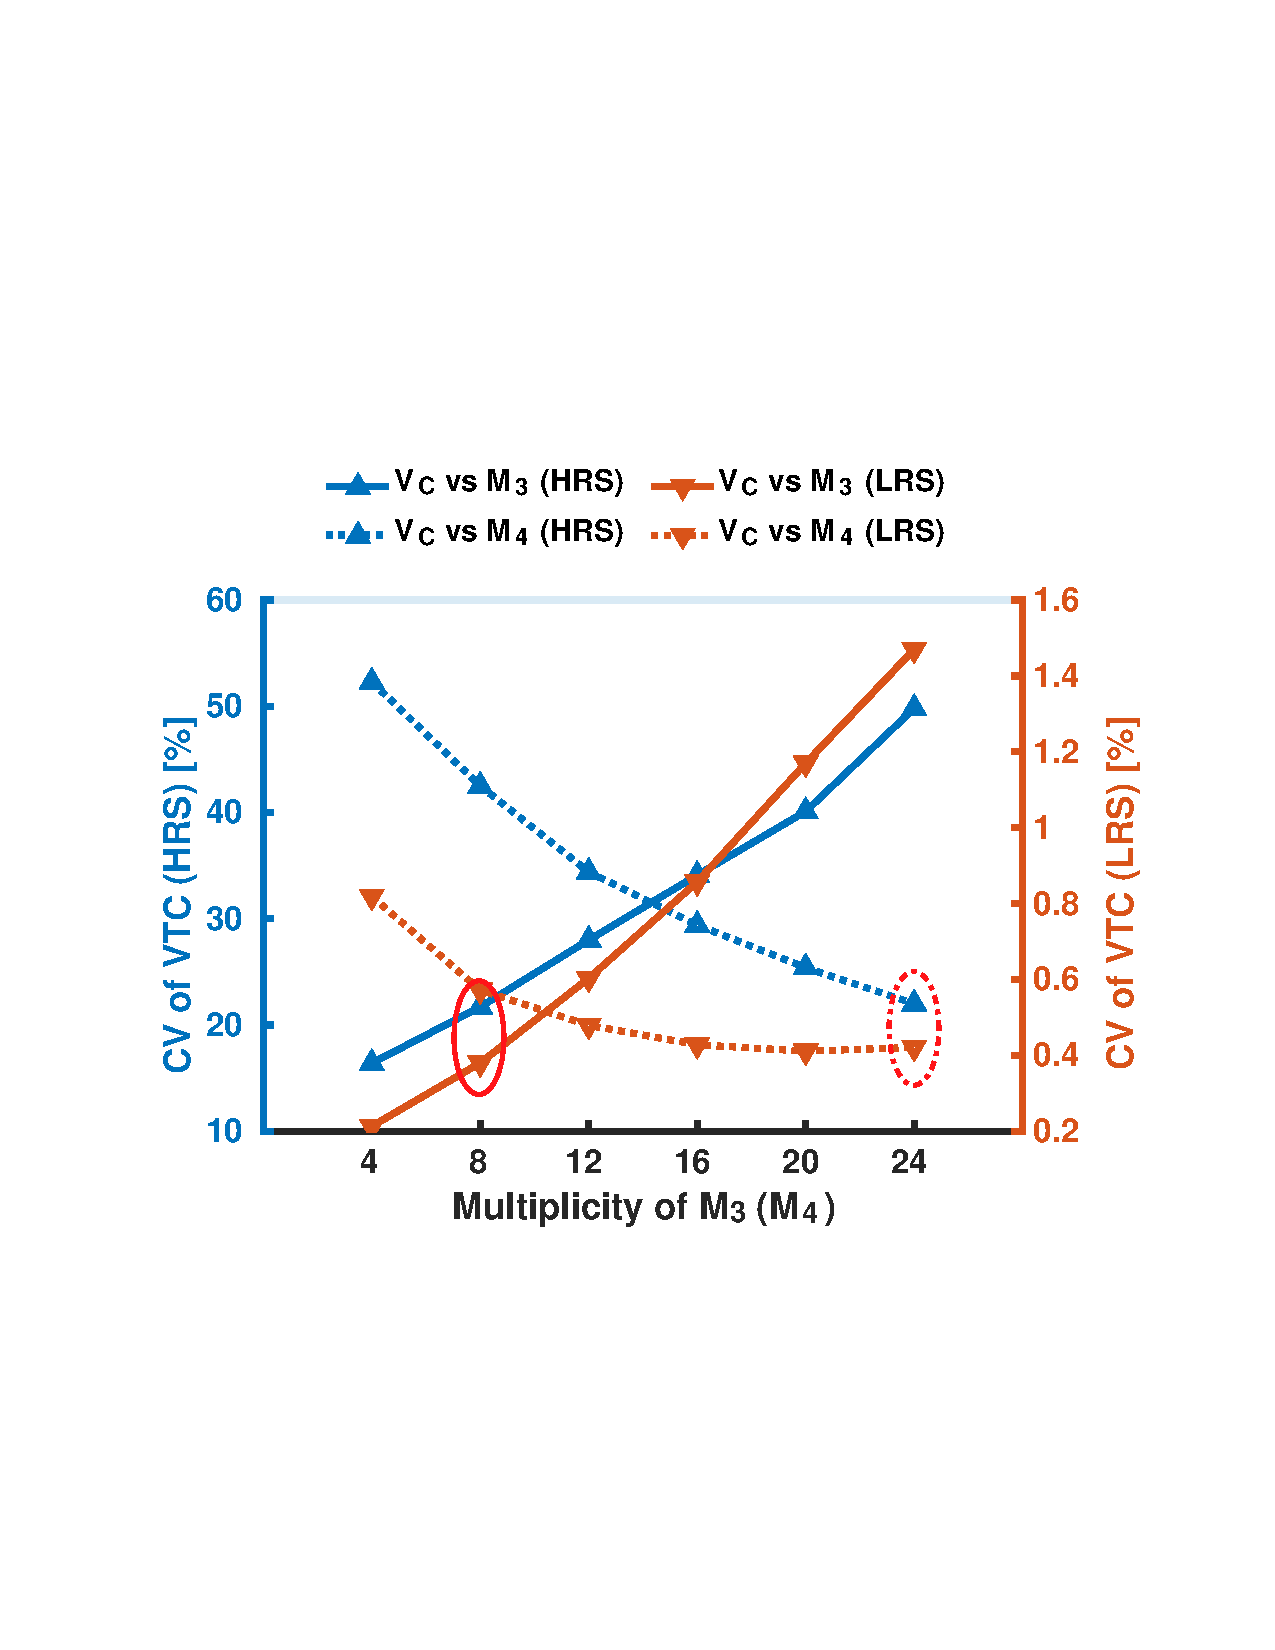
\includegraphics[width=0.44\textwidth]{fig/cv_of_vtc.pdf}}
\caption{The coefficient of variation (CV) of the VTC versus the multiplicity of $M_3$ (the $M_4$ multiplicity is set to 24) and $M_4$ (the $M_3$ multiplicity is set to 8).}
\label{fig_cv_vtc}
\end{figure}

\begin{table*}[ht!]%[htbp]
\centering
\caption{Comparison of the proposed TSA with Conventional VSA and CSA}
\label{tab_performance_comp}
\begin{threeparttable}
\begingroup
\setlength{\tabcolsep}{3pt} % Default value: 6pt
\renewcommand{\arraystretch}{1.5} % Default value: 1
\begin{tabular}{@{}m{3cm}<{\centering}m{2cm}<{\centering}m{4cm}<{\centering}m{2cm}<{\centering}m{2cm}<{\centering}m{2cm}<{\centering}@{}}
\toprule[1.5pt]
Types of SA & Structure & Reference used & BER & Read energy & Read time\tnote{*}  \\ \hline
\midrule
Conventional VSA & Latch-based & $V_{ref}=\frac{1}{2}(V_{BL,L}+V_{BL,H})$ & 6.2E-7 & 45 fJ & 6 ns\\\hline
Conventional CSA & Latch-based & $I_{ref}=\frac{1}{2}(I_{BL,L}+I_{BL,H})$ & 1.5E-6 & 96 fJ & 6 ns\\\hline
Proposed TSA & VTC-based & internal delay & 1E-10 & 49 fJ & 6 ns\\
\bottomrule[1.5pt]
\end{tabular}
% \textcolor{red}{
\begin{tablenotes}
\item[*] The precharge time and developing time are set to be same for a fair comparison of BER.
% \item[**] BER is $4\times10^{-6}$ when read time is 5 ns.
\end{tablenotes}
% }
\endgroup
\end{threeparttable}
\end{table*} 



The variation of the VTC in HRS is dominated by the variations of NMOS transistor $M_3$ and $M_4$, which determine the VTC current and the gate capacitance, respectively.
To gain an insight into the inter-dependence of robustness, performance, and energy for the RRAM sensing circuit, Fig. \ref{fig_cv_vtc} depicts the coefficient of variation of the VTC versus the multiplicity of $M_3$ (the $M_4$ multiplicity is set to 24) and $M_4$ (the $M_3$ multiplicity is set to 8). As discussed before, the CV of the VTC when RRAM is in LRS is much smaller than that when RRAM is in HRS. 
Interestingly, the trends of the curves are similar in both HRS and LRS. A larger size of $M_3$ provides a larger pull-down current of the VTC, leading to a larger voltage drop of $V_C$. On the other hand, the smaller size of $M_4$ provides lower gate capacitance, leading to a larger voltage drop of $V_C$ as well. Increasing $M_3$ and reducing $M_4$ have the same effect, both increasing the variation of the VTC. From this point of view, reducing $M_3$ and increasing $M_4$ improve the stability of the VTC. However, smaller $M_3$ takes a longer read time while larger $M_4$ occupies a significant silicon area.
% In this work, the high CV of the VTC in HRS does not affect state discrimination. As the timing graph is shown at the top of Fig. \ref{fig_cv_vtc}, the sensing margin is still large enough even though the large variations of the VTC when the RRAM is in HRS.
Unless otherwise stated, the size of $M_3$ and $M_4$ are set as $8\times$ and $24\times$, respectively, for the optimized overall performance in the other simulations.

\subsection{Comparison of the Proposed TSA to Prior Counterparts}

To compare the proposed TSA with the conventional VSA and CSA, we implemented the voltage and current latch-based VSA and CSA, respectively, in the same process. The reference voltage (current) is designed at the midpoint between two dummy bitlines when the RRAMs are in HRS and LRS respectively, resulting in a sensing margin that is equal to half of the difference between BL swings. 
Table \ref{tab_performance_comp} compares the performance of different types of SA based on the post-layout simulation of a $512 \times 512$ 1T1R array. The proposed TSA achieves a much lower read BER that is 3--4 orders of magnitude better than conventional designs, making it suitable for reliable and robust RRAM sensing.


\begin{table}[t!]%[htbp]
\centering
\caption{Feature Summary and Comparison of the Time-based Sensing with the Prior Arts}
\label{tab_performance_comparison}
\begin{threeparttable}
\begin{tabular}{@{}m{1cm}<{\centering}m{1.65cm}<{\centering}m{1.5cm}<{\centering}m{1.5cm}<{\centering}m{1.5cm}<{\centering}@{}}
\specialrule{0em}{1pt}{1pt}
\toprule[1.5pt]
Reference & Chien'18 \cite{8123866}  & Na'15 \cite{7206572} & Lu'21 \cite{9401390}  & This work \\ \hline
\midrule
Sensing scheme & Two-step charge-pump & Dual-stage sensing & Biased current sensing & Time-based sensing\\\hline
\specialrule{0em}{1pt}{1pt}
Process & 150 nm & 45 nm & 40 nm & 40 nm \\\hline
\specialrule{0em}{1pt}{1pt}
Voltage & 2 V & 1 V & 1.2 V & 1.2 V \\\hline
\specialrule{0em}{1pt}{1pt}
\makecell{HRS/\\LRS} & \makecell{10 G$\Omega$/\\0.2 G$\Omega$} & \makecell{7.5 K$\Omega$/\\ 3 K$\Omega$} & \makecell{500 K$\Omega$/\\ 10 K$\Omega$} & \makecell{500 K$\Omega$/\\ 10 K$\Omega$} \\\hline
\specialrule{0em}{1pt}{1pt}
Read time & 1.3 $\micro$s\tnote{*} & 3.4 ns & 7 ns & 6 ns\tnote{**} \\\hline
\specialrule{0em}{1pt}{1pt}
MLC sensing & No & No & No & Yes \\\hline
\specialrule{0em}{1pt}{1pt}
Advantage & Simple type, small area & Offset-canceling, fast read speed & Simple type, fast read speed & Low power, fast speed, low BER\\\hline
\specialrule{0em}{1pt}{1pt}
Drawback & Long read time & High res. sensing failure & Sensitive to PVT & Timing ctr. needs match the VTC \\
\bottomrule[1.5pt]
\end{tabular}
% \textcolor{red}{
\begin{tablenotes}
\item[*] Measured result.
\item[**] BER is $1\times10^{-10}$ when read time is 6 ns. Read time would be shorter at the cost of higher BER. 
\end{tablenotes}
% }
\end{threeparttable}
\end{table} 


Table \ref{tab_performance_comparison} reports the specifications of the proposed time-based sensing and comparisons of various RRAM sensing schemes. 
The RRAM stack in our work has a middle resistance range (tens to hundreds of kilo Ohm). By enabling the energy-intensive sensing inverter at the sensing point only, the proposed sensing scheme consumes lower energy. The voltage margin of the discharging node is enlarged by charge compensation. 
Compared with other types of sensing scheme, the time-based sensing achieves higher robustness since the read margin can be expanded easily in the time-domain. The BER is $1\times10^{-10}$ when the delay is 5 ns, as shown in Fig. \ref{fig_ber_delay}. The read BER can be reduced further by the multi-level sensing at the cost of longer read time. 
Besides, the time-based sensing scheme does not require the reference generation circuit or the auxiliary DC power supply, in contrast with other kinds of sensing schemes. This not only eliminates the effect of sensitive analog reference variation, but simplifies the readout circuit design of the RRAM memory array.
However, the proposed scheme needs to adjust the delay line for different resistance magnitudes of RRAM to optimize the overall area-speed-robustness-energy performance. 

